\chapter{वृक्क-शरीरक्रिया और परासरण-नियमन}\label{ch:b3:renal-osmoregulation}

आपके गुर्दे दिन भर में एक सौ अस्सी लीटर प्लाज़्मा छानते हैं --- यानी
हर आधे घंटे में आपके रक्त का पूरा आयतन --- और डेढ़ लीटर को छोड़कर सब
लौटा देते हैं, यूरिया निकालकर, नमक, अम्ल और जल को शरीर की ज़रूरत के
प्रतिशत भर के भीतर साधकर, और ग्लूकोस का हर ग्राम रखकर। रेगिस्तान का कोई
कंगारू चूहा कभी पीता ही नहीं: वह उसी जल पर जीता है जो उसका उपापचय सूखे
बीजों से बनाता है, और समुद्री जल से पाँच गुना गाढ़ा मूत्र निकालता है।
कोई समुद्री मछली लगातार पीती है और नमक अपने क्लोमों से बाहर पंप करती
है; कोई मीठे पानी की मछली कभी पीती ही नहीं और नमक भीतर पंप करती है। ये
सब जो समस्या हल करते हैं वह एक ही है: कोशिकाओं के चारों ओर के द्रव का
संघटन अचर रखना, जबकि खाना, पीना और साँस लेना उसे बिगाड़ते रहें, और
नाइट्रोजन इस तरह फेंकना कि बहुत अधिक जल न फिंक जाए। यह अध्याय स्तनी
गुर्दे को हल किए गए उदाहरण की तरह लेता है --- निस्यंदन, निकासी का
अंकगणित, वह प्रतिधारा-चाल जो मूत्र गाढ़ा करती है, और वे हॉर्मोन जो
सुइयाँ सेट करते हैं --- और फिर प्राणियों भर में हलों की परास।

\section{समस्या}

\begin{definition}[परासरण-नियमन]\label{def:b3:renal-osmoregulation:problem}
\index{परासरणीयता}\index{परासरण दाब}\index{बाह्यकोशिकीय द्रव}\index{परासरण-अनुरूपी}\index{परासरण-नियामक}
किसी विलयन की \emph{परासरणीयता} उसके घुले कणों की कुल सांद्रता है
(ऑस्मोल प्रति लीटर में); वही \emph{परासरण दाब} तय करती है, तनु विलयनों
के लिए $\Pi = cRT$, जो जल को हर उस झिल्ली के आर-पार चलाता है जो जल
गुज़ारे पर विलेय नहीं। किसी स्तनी के देह-द्रव लगभग \qty{300}{mOsm/L}
पर बैठते हैं --- देह-द्रव्यमान का \qty{40}{\%} कोशिकाओं के भीतर,
\qty{20}{\%} बाहर, यानी वह \emph{बाह्यकोशिकीय द्रव} जिसका चौथाई
प्लाज़्मा है --- और बाहर कुछ बदले तो कोशिकाएँ सेकंडों में फूल या सिकुड़
जाती हैं, क्योंकि उनकी झिल्लियाँ जल स्वच्छंद गुज़ारती हैं। कोई
\emph{परासरण-अनुरूपी} (अधिकांश समुद्री अकशेरुकी, शार्क) अपने द्रव
समुद्र की परासरणीयता पर रखता है और केवल उनका संघटन नियंत्रित करता है;
कोई \emph{परासरण-नियामक} (कशेरुकी, कीट, मीठे पानी के प्राणी) अपनी
परासरणीयता पर्यावरण के सामने अचर रखता है, जिसकी ऊर्जा-लागत उस प्रवणता
के समानुपाती होती है। दूसरा काम, जो पहले से जुड़ा है, प्रोटीन-विघटन की
नाइट्रोजन ठिकाने लगाना है: भरपूर जल में \emph{अमोनिया} के रूप में
(मछलियाँ), \emph{यूरिया} के रूप में, जो घुलनशील और अविषालु है पर जिसे
ढोने के लिए जल चाहिए (स्तनी), या \emph{यूरिक अम्ल} के रूप में, यानी
कोई लगभग सूखी लेई (पक्षी, सरीसृप, कीट)।
\end{definition}

\section{वृक्काणु और निस्यंदन}

\begin{definition}[वृक्काणु]\label{def:b3:renal-osmoregulation:nephron}
\index{वृक्काणु}\index{केशिकागुच्छ}\index{समीपस्थ नलिका}\index{हेनले का पाश}\index{संग्रह नलिका}
हर मानव गुर्दे में लगभग दस लाख \emph{वृक्काणु} हैं। रक्त किसी
\emph{केशिकागुच्छ} में घुसता है, यानी बोमन-संपुट के भीतर केशिकाओं के
किसी गुच्छे में, जिसकी दीवारें --- गवाक्षित अंतःस्तर, आधार कला, और
पादकोशिकाओं के पैरों के बीच के दरार-पट --- जल और लगभग \qty{60}{kDa} से
नीचे का हर विलेय गुज़ार देती हैं पर प्रोटीन तथा कोशिकाएँ रोक लेती हैं।
वह निस्यंद \emph{समीपस्थ नलिका} से होकर बहता है, जो दो-तिहाई जल तथा
नमक और सारा ग्लूकोस तथा ऐमीनो अम्ल फिर सोख लेती है; फिर \emph{हेनले के
पाश} में नीचे और ऊपर, जो मज्जा तक पहुँचता है और अगले खंड की
सांद्रता-प्रवणता बनाता है; फिर \emph{दूरस्थ नलिका} से होकर, जहाँ नमक
साधा जाता है; और \emph{संग्रह नलिका} में, जहाँ अंतिम जल-मात्रा
वैसोप्रेसिन तय करता है, जब वह नलिका मज्जा से होकर वृक्क-द्रोणी तक जाती
है। जो रक्त केशिकागुच्छ से निकलता है वह नलिकाओं के चारों ओर की किसी
दूसरी केशिका-शय्या में घुसता है, जो उनका पुनःसोखा हुआ सब ले लेती है।
\end{definition}

\begin{omfigure}
\begin{tikzpicture}[every node/.style={font=\scriptsize}, >=stealth]
  % cortex/medulla background
  \fill[omDef!6] (-0.5,0) rectangle (11.5,3.6); \fill[omProp!8] (-0.5,-3.4) rectangle (11.5,0);
  \node[right, gray] at (-0.4,3.4) {वल्कुट}; \node[right, gray] at (-0.4,-3.2) {मज्जा};
  % glomerulus
  \draw[thick, omThm, fill=omThm!20] (0.8,2.6) circle (0.55); \node[below, align=center] at (0.25,2.0) {केशिकागुच्छ:\\निस्यंदन,\\\qty{180}{L/d}};
  % proximal tubule
  \draw[very thick, omDef] (1.35,2.6) .. controls (2.2,3.3) and (2.8,2.0) .. (3.2,2.6) .. controls (3.5,3.1) and (3.9,2.2) .. (4.2,2.6);
  \node[below, align=center] at (2.65,2.05) {समीपस्थ नलिका:\\Na$^{+}$ तथा जल का \qty{67}{\%},\\सारा ग्लूकोस, ऐमीनो अम्ल,\\HCO$_3^-$};
  % loop of Henle
  \draw[very thick, omDef] (4.2,2.6) -- (4.2,-2.8) arc[start angle=180, end angle=360, radius=0.4] -- (5.0,2.6);
  \node[left, align=right] at (4.1,-1.0) {अवरोही भुजा:\\जल निकलता है};
  \node[right, align=left] at (5.1,-1.6) {आरोही भुजा:\\NaCl पंप होता है,\\जल नहीं};
  \node[right, align=left, omProp!80!black] at (5.1,-0.2) {Na$^{+}$ का \qty{25}{\%}};
  % distal tubule
  \draw[very thick, omDef] (5.0,2.6) .. controls (5.4,3.2) and (6.0,2.0) .. (6.4,2.6) .. controls (6.8,3.1) .. (7.2,2.6);
  \node[above, align=center] at (6.0,3.1) {दूरस्थ नलिका: Na$^{+}$ (ऐल्डोस्टेरॉन),\\Ca$^{2+}$, K$^{+}$ का स्राव};
  % collecting duct
  \draw[very thick, omMeth!70!black] (7.2,2.6) -- (7.8,2.6) -- (7.8,-3.2);
  \node[right, align=left] at (7.9,-1.2) {संग्रह नलिका:\\जल (वैसोप्रेसिन,\\ऐक्वापोरिन-2),\\यूरिया, H$^{+}$;\\\qty{1.5}{L/d} बाहर};
  \draw[->, thick, omMeth!70!black] (7.8,-3.2) -- (7.8,-3.6);
  % osmolarity scale on the right
  \foreach \y/\c in {2.6/300, 0.0/600, -1.4/900, -2.8/1200} { \node[left, omProp!80!black, font=\tiny] at (11.4,\y) {\c\ mOsm}; }
  \draw[->, omProp!80!black] (11.4,2.9) -- (11.4,-3.1); \node[above, omProp!80!black, font=\tiny, align=center] at (11.4,3.0) {अंतराली\\परासरणीयता};
\end{tikzpicture}

{\small बिछाया हुआ कोई \omterm{def:b3:renal-osmoregulation:nephron}{वृक्काणु}। वल्कुट में निस्यंदन; \omterm{def:b3:renal-osmoregulation:nephron}{समीपस्थ नलिका} में
थोक पुनःसोखन; \omterm{def:b3:renal-osmoregulation:nephron}{हेनले का पाश} मज्जा में डुबकी लगाता हुआ, जहाँ अंतराल गहराई
के साथ अधिक नमकीन होता जाता है; और \omterm{def:b3:renal-osmoregulation:nephron}{संग्रह नलिका} उसी प्रवणता से होकर
वापस जाती हुई, जो वैसोप्रेसिन की छूट हो तो जल छोड़ देती है।}
\end{omfigure}

\begin{theorem}[निस्यंदन और निकासी]\label{thm:b3:renal-osmoregulation:clearance}
\index{स्टार्लिंग बल}\index{केशिकागुच्छी निस्यंदन दर}\index{निकासी}\index{इनुलिन}\index{क्रिएटिनिन}
निस्यंद केशिकागुच्छी दीवार के आर-पार किसी ऐसी दर से बहता है जो
\emph{\omterm{thm:b3:renal-osmoregulation:clearance}{स्टार्लिंग बल}} तय करते हैं: केशिका का द्रवस्थैतिक दाब
$P_{\text{GC}}$ तरल को बाहर धकेलता है, बोमन-अवकाश का द्रवस्थैतिक दाब
$P_{\text{BS}}$ और प्लाज़्मा प्रोटीनों का कलिलाकर्षी दाब
$\pi_{\text{GC}}$ उसे वापस खींचते हैं, और
\[
\text{GFR} = K_{f}\,\bigl(P_{\text{GC}} - P_{\text{BS}} - \pi_{\text{GC}}\bigr)
\approx K_{f}\,(55 - 15 - 30)\ \unit{mmHg} = K_{f}\times \qty{10}{mmHg},
\]
यानी \emph{\omterm{thm:b3:renal-osmoregulation:clearance}{केशिकागुच्छी निस्यंदन दर}}, जो किसी वयस्क में लगभग
\qty{125}{mL/min} है। किसी भी पदार्थ $x$ के लिए, जिसकी प्लाज़्मा
सांद्रता $P_{x}$ हो, मूत्र-सांद्रता $U_{x}$ और मूत्र-प्रवाह $V$,
\emph{निकासी}
\[
C_{x} = \frac{U_{x}\,V}{P_{x}}
\]
प्लाज़्मा का वह आयतन है जो प्रति एकांक समय $x$ से साफ़ होता है। यदि
$x$ स्वच्छंद छना हो और न पुनःसोखा जाए न स्रवित (इनुलिन, और लगभग वैसा ही
क्रिएटिनिन), तो $C_{x} = \text{GFR}$; यदि वह गुर्दे से गुज़रते
प्लाज़्मा से पूरी तरह हटा दिया जाए (कम मात्रा में पैरा-अमीनोहिप्यूरेट),
तो $C_{x}$ वृक्कीय प्लाज़्मा प्रवाह के बराबर है; GFR से कम निकासी का
अर्थ शुद्ध पुनःसोखन है, उससे अधिक का शुद्ध स्राव, और छना भार
$\text{GFR}
\times P_{x}$ में से उत्सर्जन $U_{x}V$ घटाने पर पुनःसोखी गई मात्रा
मिलती है।
\end{theorem}
\begin{proof}
निस्यंदन किसी छिद्रित दीवार से होकर अति-निस्यंदन है: प्रवाह उसके
आर-पार के शुद्ध दाब के समानुपाती है, और शुद्ध दाब बाहर की ओर का
द्रवस्थैतिक दाब घटा भीतर की ओर के द्रवस्थैतिक तथा कलिलाकर्षी दाब है
(स्टार्लिंग), क्योंकि निस्यंद का कलिलाकर्षी दाब नगण्य है, उसमें कोई
प्रोटीन नहीं। निकासी: एकांक समय में गुर्दा $U_{x}V$ जितना $x$ उत्सर्जित
करता है; प्लाज़्मा का जो आयतन इतनी मात्रा रखता था वह $U_{x}V/P_{x}$
है। जो पदार्थ केवल छना जाए, उसके लिए जो उत्सर्जित होता है वही छना था,
$\text{GFR}\times P_{x} = U_{x}V$, जिससे $C_{x} = \text{GFR}$। जो पूरी
तरह निकाल लिया जाए, उसके लिए बहते प्लाज़्मा का सारा $x$, यानी
$\text{RPF}\times P_{x}$, उत्सर्जित होता है, जिससे
$C_{x} = \text{RPF}$। द्रव्यमान-संतुलन पुनःसोखी मात्रा दे देता है।
\end{proof}

\begin{example}[संख्याओं में निकासियाँ]\label{ex:b3:renal-osmoregulation:numbers}
\qty{1}{mg/mL} के प्लाज़्मा स्तर तक चढ़ाया गया इनुलिन मूत्र में
\qty{125}{mg/mL} पर, \qty{1}{mL/min} के प्रवाह के साथ प्रकट होता है:
$C = 125\times 1/1 =
\qty{125}{mL/min}$, यानी GFR, \qty{180}{L/d}। पैरा-अमीनोहिप्यूरेट
\qty{650}{mL/min} देता है, यानी प्लाज़्मा प्रवाह; $0.45$ के हीमैटोक्रिट
के साथ वृक्कीय रक्त-प्रवाह \qty{1.2}{L/min} है, यानी देह-द्रव्यमान के
\qty{0.5}{\%} के लिए हृद्-निर्गम का पाँचवाँ भाग, और निस्यंदन-अंश
$125/650 = 0.19$। यूरिया: प्लाज़्मा \qty{5}{mmol/L}, मूत्र
\qty{300}{mmol/L}, \qty{1}{mL/min} पर --- निकासी \qty{60}{mL/min},
यानी GFR की आधी, इसलिए छनी यूरिया की आधी पुनःसोख ली जाती है। ग्लूकोस:
सामान्य प्लाज़्मा स्तरों पर निकासी शून्य, दिन भर में छने \qty{180}{g}
का हर अणु लौटा हुआ। क्रिएटिनिन, जो पेशी किसी अचर दर से बनाती है और जो
केवल छना जाता है, चिकित्सालय का GFR-माप है: GFR आधी होने पर प्लाज़्मा
क्रिएटिनिन दुगुना हो जाता है, बिना मूत्र इकट्ठा किए।
\end{example}

\begin{method}[गुर्दे का प्रकार्य नापना]\label{met:b3:renal-osmoregulation:gfr}
\index{GFR का मापन}
(1) किसी शोध-मान के लिए, इनुलिन किसी स्थिर प्लाज़्मा स्तर तक चढ़ाइए,
समयबद्ध मूत्र इकट्ठा कीजिए, दोनों नापिए, और $UV/P$ निकालिए।
(2) चिकित्सालय में, प्लाज़्मा क्रिएटिनिन नापिए और उससे GFR का आकलन किसी
ऐसे सूत्र से कीजिए जो आयु, लिंग और देह-आकार का सुधार करे; उसी आकलन से
चिरकारी वृक्क रोग की अवस्थाएँ परिभाषित होती हैं (तीन महीने तक
\qty{60}{mL/min} से नीचे GFR)। (3) मूत्र में ऐल्ब्युमिन नापकर उस छन्ने
की वरणशीलता जाँचिए --- सामान्यतः \qty{30}{mg/d} से कम; उससे अधिक का
अर्थ है कोई रिसता अवरोध, यानी मधुमेही वृक्क-क्षति का सबसे आरंभिक चिह्न।
(4) रात भर जल रोककर और मूत्र की \omterm{def:b3:renal-osmoregulation:problem}{परासरणीयता} नापकर गाढ़ा करने की क्षमता
जाँचिए, जो \qty{800}{mOsm/L} से ऊपर होनी चाहिए; सामान्य GFR के साथ
गाढ़ा न कर पाना \omterm{def:b3:renal-osmoregulation:nephron}{संग्रह नलिका} या वैसोप्रेसिन की ओर इशारा करता है।
\end{method}

\begin{omfigure}
\begin{tikzpicture}
\begin{axis}[
  width=0.68\linewidth, height=5.6cm,
  axis x line=bottom, axis y line=left,
  xmin=0, xmax=800, ymin=0, ymax=700,
  xlabel={प्लाज़्मा ग्लूकोस (mg/dL)}, ylabel={mg/min},
  xlabel style={font=\small, at={(axis description cs:0.5,-0.12)}, anchor=north}, ylabel style={font=\small},
  tick label style={font=\small}, xtick={0,100,200,300,400,600,800}, ytick={0,200,375,600},
  clip=false,
]
\addplot[very thick, omDef, domain=0:800, samples=2] {1.25*x};
\addplot[very thick, omMeth!70!black, domain=0:200, samples=2] {1.25*x};
\addplot[very thick, omMeth!70!black, smooth] coordinates {(200,250) (250,300) (300,340) (350,365) (400,375) (800,375)};
\addplot[very thick, omThm, domain=0:180, samples=2] {0};
\addplot[very thick, omThm, smooth] coordinates {(180,0) (250,12) (300,35) (350,72) (400,125) (800,625)};
\draw[dashed, gray] (axis cs:180,0) -- (axis cs:180,700); \node[font=\scriptsize, gray, anchor=north west] at (axis cs:185,560) {देहली};
\draw[dashed, gray] (axis cs:0,375) -- (axis cs:800,375);
\node[font=\scriptsize, omDef, anchor=south east] at (axis cs:480,620) {छना: GFR $\times$ P};
\node[font=\scriptsize, omMeth!70!black, anchor=south west, align=left] at (axis cs:660,395) {पुनःसोखा:\\$T_{m} = \qty{375}{mg/min}$};
\node[font=\scriptsize, omThm, anchor=north west] at (axis cs:520,300) {उत्सर्जित};
\end{axis}
\end{tikzpicture}

{\small ग्लूकोस का अनुमापन वक्र। छना भार प्लाज़्मा स्तर के साथ चढ़ता
है; \omterm{def:b3:renal-osmoregulation:nephron}{समीपस्थ नलिका} के वाहक उसे अपनी अधिकतम $T_{m}$ तक पूरा पुनःसोख लेते
हैं; उस देहली के ऊपर, जो लगभग \qty{180}{mg/dL} (\qty{10}{mmol/L}) पर
है, ग्लूकोस मूत्र में छलक जाता है --- यानी अनुपचारित मधुमेह के मूत्र की
वह शर्करा।}
\end{omfigure}

\section{मूत्र को गाढ़ा करना}

\begin{proposition}[प्रतिधारा गुणक]\label{prop:b3:renal-osmoregulation:countercurrent}
\index{प्रतिधारा गुणन}\index{एकल प्रभाव}\index{वैसोप्रेसिन}\index{ऐक्वापोरिन}\index{यूरिया का पुनर्चक्रण}
\omterm{def:b3:renal-osmoregulation:nephron}{हेनले का पाश} वल्कुट पर \qty{300}{mOsm/L} से मज्जा की नोक पर
\qty{1200}{mOsm/L} तक \omterm{def:b3:renal-osmoregulation:problem}{परासरणीयता} की कोई प्रवणता बना देता है, और इसमें
कोई भी कोशिका उसके किसी अंश से अधिक के विरुद्ध पंप नहीं करती। मोटी
आरोही भुजा अपने तरल से NaCl निकालकर अंतराल में पंप करती है और जल के
लिए अपारगम्य है, इसलिए हर स्तर पर वह अंतराल को अपनी अंतर्वस्तु से लगभग
\qty{200}{mOsm/L} अधिक नमकीन बना देती है --- यही \emph{\omterm{prop:b3:renal-osmoregulation:countercurrent}{एकल प्रभाव}} है।
अवरोही भुजा जल के लिए पारगम्य है और अंतराल के साथ संतुलित हो जाती है,
इसलिए नीचे बहता तरल उतरते-उतरते अधिक नमकीन होता जाता है और मोड़ पर कोई
पहले से गाढ़ा तरल पहुँचा देता है, जिससे फिर आरोही भुजा पंप करती है; और
ऊपर बहता तरल हर स्तर पर अंतराल से अधिक तनु होता जाता है और उस पाश से
\qty{100}{mOsm/L} पर, अल्पपरासरणी, निकलता है। प्रतिधारा प्रवाह किसी छोटे
अनुप्रस्थ प्रभाव को किसी बड़ी अनुदैर्घ्य प्रवणता में बदल देता है: मोड़
का सबसे नमकीन तरल उस तरल से बना था जो पहले ही नमकीन था, चरण-दर-चरण।
फिर \omterm{def:b3:renal-osmoregulation:nephron}{संग्रह नलिका} इसी प्रवणता से होकर नीचे उतरती है।
\emph{वैसोप्रेसिन} (मूत्ररोधी हॉर्मोन) के बिना उसकी दीवार जल के लिए
अपारगम्य है और हर घंटे लीटर भर या उससे अधिक तनु मूत्र निकलता है; उसके
साथ, अवकाशिकीय झिल्ली में \emph{ऐक्वापोरिन-2} वाहिकाएँ ठेल दी जाती हैं,
जल उस प्रवणता के सहारे मज्जा में निकल जाता है, और वह मूत्र नोक की
\omterm{def:b3:renal-osmoregulation:problem}{परासरणीयता}, \qty{1200}{mOsm/L}, तक पहुँच जाता है। यूरिया, जो भीतरी
नलिका से पुनःसोखी जाती है और मज्जा में फँस जाती है, नोक की \omterm{def:b3:renal-osmoregulation:problem}{परासरणीयता}
का आधा जुटाती है, और वासा रेक्टा, जो स्वयं प्रतिधारा में हैं, पुनःसोखा
गया जल उस प्रवणता को बहाए बिना हटा देती हैं।
\end{proposition}

\begin{proof}[प्रमाण-सामग्री]
विर्ट्ज़, हार्गिताई और कुन (1951) ने चूहों के गुर्दे जमाए और वल्कुट से
अंकुरिका तक की काटों के तरल का गलनांक नापा: \omterm{def:b3:renal-osmoregulation:problem}{परासरणीयता} गहराई के साथ
लगातार चढ़ती गई और नोक पर मूत्र के मान तक पहुँची --- यानी वही प्रवणता
जो प्रतिधारा गुणक के सिद्धांत (कुन, जो भौतिक रसायनज्ञ था, 1942) ने
माँगी थी। फिर नलिकाओं के सूक्ष्म-वेधन (गॉट्सचॉक, 1959) ने पाश के मोड़
का तरल अतिपरासरणी और आरोही भुजा से निकलता तरल अल्पपरासरणी पाया, और
वैसोप्रेसिन मौजूद होने पर \omterm{def:b3:renal-osmoregulation:nephron}{संग्रह नलिका} का तरल हर स्तर पर अंतराल से मेल
खाता। सबसे लंबे पाशों वाले रेगिस्तानी कृंतकों की प्रवणताएँ सबसे तीखी
थीं और मूत्र सबसे गाढ़ा।
\end{proof}

\begin{omfigure}
\begin{tikzpicture}[every node/.style={font=\scriptsize}, >=stealth]
  % loop
  \draw[very thick, omDef] (0,3.2) -- (0,-0.4) arc[start angle=180, end angle=360, radius=0.7] -- (1.4,3.2);
  \draw[very thick, omDef] (0.35,3.2) -- (0.35,-0.4) arc[start angle=180, end angle=360, radius=0.35] -- (1.05,3.2);
  % interstitial osmolarity bands
  \foreach \y/\c/\col in {2.8/300/10, 2.0/500/25, 1.2/700/40, 0.4/900/55, -0.4/1100/70, -1.0/1200/80} { \fill[omProp!\col, opacity=0.5] (-2.2,\y-0.4) rectangle (-0.2,\y+0.4); \node[left, font=\tiny] at (-2.25,\y) {\c}; }
  \node[left, align=right, font=\tiny] at (-2.25,3.35) {अंतराल\\(mOsm/L)};
  % arrows: water out of descending, NaCl out of ascending
  \foreach \y in {2.4,1.6,0.8,0.0} { \draw[->, thick, omDef!70!black] (0.15,\y) -- (-0.4,\y); }
  \node[left, omDef!70!black, font=\tiny] at (-0.45,2.4) {H$_2$O};
  \foreach \y in {2.4,1.6,0.8,0.0} { \draw[->, thick, omThm] (1.25,\y) -- (1.9,\y); }
  \node[right, omThm, font=\tiny] at (1.5,2.85) {NaCl पंप};
  % fluid osmolarity labels inside limbs
  \node[above] at (0.17,3.25) {\qty{300}{} भीतर}; \node[above] at (1.22,3.25) {\qty{100}{} बाहर};
  \node[font=\tiny] at (0.7,-1.35) {मोड़ पर 1200};
  \node[below, align=center] at (0.2,-1.7) {अवरोही भुजा: जल निकलता है,\\तरल गाढ़ा होता है; आरोही भुजा:\\नमक निकलता है, तरल तनु होता है};
  % collecting duct
  \draw[very thick, omMeth!70!black] (4.2,3.2) -- (4.2,-1.4); \node[above, align=center] at (4.2,3.25) {संग्रह नलिका};
  \foreach \y in {2.4,1.6,0.8,0.0,-0.8} { \draw[->, thick, omMeth!70!black] (4.1,\y) -- (3.5,\y); }
  \node[right, align=left, font=\tiny] at (4.3,1.2) {वैसोप्रेसिन के साथ:\\ऐक्वापोरिन-2 ठेला गया,\\जल प्रवणता के सहारे\\निकल जाता है};
  \node[below, align=center] at (4.2,-1.5) {मूत्र\\\qty{1200}{mOsm/L} तक};
  % single effect note
  \node[right, align=left] at (6.4,2.6) {एकल प्रभाव: आरोही भुजा अंतराल को हर स्तर पर\\अपने ही तरल से $\sim\qty{200}{mOsm/L}$\\ऊपर रखती है;\\प्रतिधारा प्रवाह इन प्रभावों को वल्कुट से\\अंकुरिका तक \qty{900}{mOsm/L} की\\किसी प्रवणता में चुन देता है};
\end{tikzpicture}

{\small प्रतिधारा गुणक। आरोही भुजा से पंप किया गया नमक अंतराल को
अतिपरासरणी बना देता है; अवरोही भुजा से खींचा गया जल उस तरल को पंप तक
पहुँचने से पहले गाढ़ा कर देता है; और उलटी दिशाओं का प्रवाह किसी छोटे
अनुप्रस्थ अंतर को चार गुनी प्रवणता में चुन देता है, जिसे \omterm{def:b3:renal-osmoregulation:nephron}{संग्रह नलिका}
तब मूत्र गाढ़ा करने में काम में लेती है जब वैसोप्रेसिन उसे जल के लिए
खोल दे।}
\end{omfigure}

\begin{proposition}[जल का अंकगणित]\label{prop:b3:renal-osmoregulation:water}
\index{अनिवार्य जल-हानि}\index{मुक्त-जल निकासी}
जिस शरीर को रोज़ाना कोई विलेय-भार $S$ (लगभग \qty{600}{mOsm}, अधिकांश
यूरिया और नमक) किसी अधिकतम मूत्र-परासरणीयता $U_{\max}$ पर उत्सर्जित
करना हो उसे कोई न्यूनतम मूत्र-आयतन $V_{\min} = S/U_{\max}$ चाहिए: किसी
मनुष्य के लिए, दिन भर में $600/1200 = \qty{0.5}{L}$, यानी
\emph{अनिवार्य} जल-हानि, जिसमें फुफ्फुस तथा त्वचा लगभग \qty{0.9}{L} और
जोड़ देते हैं। समुद्री जल पीना (लगभग \qty{1000}{mOsm/L}, जिसका लगभग
सारा नमक है) लीटर भर जल के साथ \qty{1000}{mOsm} नमक जुटाता है, जिसे
उत्सर्जित करना ही पड़ेगा; $U_{\max}$ पर उसमें
$1000/1200 = \qty{0.83}{L}$ मूत्र लगता है, पर वह नमक किसी यूरिया-भार के
साथ भी उत्सर्जित होता है, और शुद्ध लाभ शून्य के पास या ऋणात्मक होता है:
समुद्री जल पीता कोई जहाज़-भग्न नाविक न पीने वाले से तेज़ निर्जलित होता
है। \emph{\omterm{prop:b3:renal-osmoregulation:water}{मुक्त-जल निकासी}}, $V - U_{\text{osm}}V/P_{\text{osm}}$,
विलेय-रहित जल का वह आयतन है जो गुर्दा प्रति एकांक समय शरीर में जोड़ता
या उससे हटाता है: किसी जल-भार में धनात्मक (तनु मूत्र), निर्जलन में
ऋणात्मक।
\end{proposition}
\begin{proof}
विलेय केवल मूत्र में निकलता है (पसीना छोड़कर), अधिक से अधिक
$U_{\max}$ सांद्रता पर, इसलिए $S = U V \le U_{\max}V$ से
$V \ge S/U_{\max}$ मिलता है। समुद्री जल के लिए: लीटर भर
\qty{1000}{mOsm} लाता है; उन्हें \qty{1200}{mOsm/L} पर उत्सर्जित करने
में \qty{0.83}{L} लगते हैं, जिससे \qty{0.17}{L} बचता है, और यह उस दिन
के अपने \qty{600}{mOsm} उपापचयी विलेय को गिनने से पहले, जिसका उत्सर्जन
उसे चुका देता है। \omterm{prop:b3:renal-osmoregulation:water}{मुक्त-जल निकासी}: आयतन $V$ और \omterm{def:b3:renal-osmoregulation:problem}{परासरणीयता}
$U_{\text{osm}}$ के मूत्र में विलेय $U_{\text{osm}}V$ है, जो प्लाज़्मा
की \omterm{def:b3:renal-osmoregulation:problem}{परासरणीयता} पर $U_{\text{osm}}V/P_{\text{osm}}$ घेरता; बाकी आयतन उससे
अधिक जल है, जो शरीर से हटा दिया गया।
\end{proof}

\begin{omfigure}
\begin{tikzpicture}
\begin{axis}[
  width=0.66\linewidth, height=5.4cm,
  axis x line=bottom, axis y line=left,
  xmin=0, xmax=1300, ymin=0, ymax=12,
  xlabel={मूत्र की परासरणीयता (mOsm/L)}, ylabel={मूत्र का आयतन (L/दिन)},
  xlabel style={font=\small, at={(axis description cs:0.5,-0.12)}, anchor=north}, ylabel style={font=\small},
  tick label style={font=\small}, xtick={50,300,600,1200}, ytick={0.5,2,6,12},
  clip=false,
]
\addplot[very thick, omDef, domain=50:1300, samples=100] {600/x};
\draw[dashed, gray] (axis cs:300,0) -- (axis cs:300,2); \draw[dashed, gray] (axis cs:1200,0) -- (axis cs:1200,0.5);
\node[font=\scriptsize, omDef, anchor=south west] at (axis cs:350,3.5) {$V = S/U$, जिसमें $S = \qty{600}{mOsm/d}$};
\node[font=\scriptsize, anchor=west, align=left] at (axis cs:1210,1.7) {अधिकतम सांद्रण:\\\qty{0.5}{L}};
\node[font=\scriptsize, anchor=south west] at (axis cs:60,9) {अधिकतम तनुकरण (\qty{50}{mOsm/L}): \qty{12}{L}};
\end{axis}
\end{tikzpicture}

{\small दिन भर का विलेय ढोने के लिए ज़रूरी मूत्र का आयतन, उसकी
सांद्रता के सामने। सबसे तनु मूत्र से, जो गुर्दा बना सकता है, सबसे गाढ़े
तक, वह आयतन चौबीस गुने की परास में फैला है; और वैसोप्रेसिन वह बिंदु
चुनता है।}
\end{omfigure}

\section{नियमन}

\begin{definition}[नियंत्रण]\label{def:b3:renal-osmoregulation:controls}
\index{रेनिन--ऐंजियोटेंसिन--ऐल्डोस्टेरॉन तंत्र}\index{ऐल्डोस्टेरॉन}\index{आलिंदी नैट्रियूरेटिक पेप्टाइड}\index{परासरण-ग्राही}\index{नलिका-केशिकागुच्छी पुनर्भरण}
दो चर अलग-अलग नियंत्रित होते हैं: \omterm{def:b3:renal-osmoregulation:problem}{बाह्यकोशिकीय द्रव} का \emph{आयतन},
जो इस बात की बात है कि शरीर कितना सोडियम थामे है, और उसकी
\emph{\omterm{def:b3:renal-osmoregulation:problem}{परासरणीयता}}, जो जल की बात है। आयतन: उपकेशिकागुच्छी उपकरण की
कोशिकाएँ, जहाँ दूरस्थ नलिका अपने ही \omterm{def:b3:renal-osmoregulation:nephron}{केशिकागुच्छ} की अणुधमनी को छूती है,
धमनी दाब या नलिका का नमक गिरने पर \emph{रेनिन} छोड़ती हैं; रेनिन किसी
प्लाज़्मा प्रोटीन से ऐंजियोटेंसिन~I काटता है, और परिवर्तक एंज़ाइम
\emph{ऐंजियोटेंसिन~II} बनाती है, जो अणुधमनियाँ सिकोड़ता है, प्यास
उद्दीप्त करता है, और अधिवृक्क वल्कुट से \emph{ऐल्डोस्टेरॉन} छुड़ाता
है, जो घंटों में दूरस्थ नलिका तथा \omterm{def:b3:renal-osmoregulation:nephron}{संग्रह नलिका} से सोडियम पुनःसोखवाता
(वाहिका ENaC के ज़रिए) और पोटैशियम स्रवित करवाता है। खिंचे हुए आलिंद
\emph{नैट्रियूरेटिक पेप्टाइड} छोड़ते हैं, जो उलटा करता है।
\omterm{def:b3:renal-osmoregulation:problem}{परासरणीयता}: अधश्चेतक के \emph{परासरण-ग्राही} \qty{1}{\%} की बढ़त भाँप
लेते हैं और मिनटों के भीतर पश्च पीयूष से वैसोप्रेसिन छुड़ाते हैं, तथा
प्यास चलाते हैं; कोई गिरावट उसे बंद कर देती है। गुर्दा अपना नियमन भी
करता है: \emph{नलिका-केशिकागुच्छी पुनर्भरण} उस \omterm{def:b3:renal-osmoregulation:nephron}{वृक्काणु} की अणुधमनी
सिकोड़ देता है जिसका दूरस्थ नमक-वितरण बहुत ऊँचा हो, जिससे हर \omterm{def:b3:renal-osmoregulation:nephron}{वृक्काणु}
का निस्यंदन उतना ही रहे जितना उसकी नलिका सँभाल सके। और अम्ल--क्षार:
\omterm{def:b3:renal-osmoregulation:nephron}{समीपस्थ नलिका} छना बाइकार्बोनेट वापस पा लेती है, \omterm{def:b3:renal-osmoregulation:nephron}{संग्रह नलिका} हज़ार गुनी
प्रवणता के विरुद्ध प्रोटॉन स्रवित करती है और उन्हें फ़ॉस्फ़ेट पर
बफ़रित करके और, सबसे बढ़कर, ग्लूटामीन से बने अमोनियम के रूप में
उत्सर्जित करती है --- यानी प्रोटीन-धनी आहार के अम्ल को ठिकाने लगाने का
शरीर का रास्ता।
\end{definition}

\begin{omfigure}
\begin{tikzpicture}[every node/.style={font=\scriptsize}, >=stealth]
  \node[draw, thick, rounded corners, fill=omThm!20, align=center] (low) at (0,0) {कम धमनी दाब\\या कम नलिकीय NaCl};
  \node[draw, thick, rounded corners, fill=omDef!20, align=center] (ren) at (3.6,0) {उपकेशिकागुच्छी\\कोशिकाएँ रेनिन छोड़ती हैं};
  \node[draw, thick, rounded corners, fill=omDef!20, align=center] (ang) at (7.4,0) {ऐंजियोटेंसिन I $\to$ II\\(परिवर्तक एंज़ाइम)};
  \node[draw, thick, rounded corners, fill=omMeth!25, align=center] (ald) at (11.0,1.2) {ऐल्डोस्टेरॉन:\\Na$^{+}$ रुका, K$^{+}$ गया};
  \node[draw, thick, rounded corners, fill=omMeth!25, align=center] (vc) at (11.0,-0.3) {अणुधमनियाँ सिकुड़तीं};
  \node[draw, thick, rounded corners, fill=omMeth!25, align=center] (th) at (11.0,-1.8) {प्यास, वैसोप्रेसिन};
  \draw[->, thick] (low) -- (ren); \draw[->, thick] (ren) -- (ang);
  \draw[->, thick] (ang) -- (ald.west); \draw[->, thick] (ang) -- (vc.west); \draw[->, thick] (ang) -- (th.west);
  \node[draw, thick, rounded corners, fill=omProp!25, align=center] (res) at (6.8,-2.6) {आयतन और दाब लौटे};
  \draw[->, thick] (ald.east) -- ++(0.4,0) |- (res.east); \draw[thick] (vc.east) -- ++(0.4,0); \draw[thick] (th.east) -- ++(0.4,0);
  \draw[-|, thick, omThm] (res.south) -- ++(0,-0.6) -| (low.south) node[pos=0.3, below, font=\tiny] {ऋणात्मक पुनर्भरण};
  \node[draw, thick, rounded corners, fill=gray!15, align=center, font=\tiny] (anp) at (2.4,-2.6) {खिंचे आलिंद: नैट्रियूरेटिक\\पेप्टाइड, उलटा};
  \draw[-|, thick, gray!60!black] (anp.east) -- (res.west);
\end{tikzpicture}

{\small रेनिन--ऐंजियोटेंसिन--ऐल्डोस्टेरॉन पाश, यानी शरीर के सोडियम का
और इसलिए उसके बाह्यकोशिकीय आयतन का धीमा नियंत्रक। ऐंजियोटेंसिन~II
वाहिकाओं, अधिवृक्क, मस्तिष्क और गुर्दे पर एक साथ काम करता है; और खिंचे
हुए हृदय से आता नैट्रियूरेटिक पेप्टाइड उसका विरोध करता है।}
\end{omfigure}

\begin{example}[दो दिन]\label{ex:b3:renal-osmoregulation:two-days}
बिना जल का एक दिन: प्लाज़्मा की \omterm{def:b3:renal-osmoregulation:problem}{परासरणीयता} $290$ से
\qty{295}{mOsm/L} की ओर चढ़ती है, वैसोप्रेसिन मिनटों में चढ़ता है,
\omterm{def:b3:renal-osmoregulation:nephron}{संग्रह नलिकाएँ} जल के लिए खुलती हैं, मूत्र गाढ़ा होकर
\qty{1200}{mOsm/L} पर आता है और आधा लीटर रह जाता है; उस व्यक्ति को प्यास
लगती है; और जो आयतन जाता है वह अधिकांशतः कोशिकाओं से जाता है, जिनका जल
बाह्यकोशिकीय नमक के पीछे चलता है। एक ही बार में पिया गया लीटर भर जल:
\omterm{def:b3:renal-osmoregulation:problem}{परासरणीयता} \qty{1}{\%} गिरती है, वैसोप्रेसिन बीस मिनटों में शून्य पर
आ जाता है, वे नलिकाएँ बंद हो जाती हैं, और अगले दो घंटों में गुर्दा
\qty{50}{mOsm/L} पर लीटर भर मूत्र निकाल देता है। लीटर भर का कोई
रक्तस्राव: दाब गिरता है, रेनिन और वैसोप्रेसिन दोनों चढ़ते हैं (आयतन
\omterm{def:b3:renal-osmoregulation:problem}{परासरणीयता} पर भारी पड़ता है), अणुधमनियाँ सिकुड़ती हैं, सोडियम तथा जल
रोके जाते हैं, और दिन भर में प्लाज़्मा का आयतन फिर भर जाता है --- पहले
अंतराल से खींचे गए और फिर पिए गए तरल से। डायबिटीज़ इन्सिपिडस, यानी
वैसोप्रेसिन या उसके ग्राही की अनुपस्थिति, दिन भर में \qty{15}{L} तनु
मूत्र और उससे मेल खाती प्यास पैदा करती है; और वृक्क-विफलता, यानी
निस्यंदन की अनुपस्थिति, ऐसा शरीर छोड़ जाती है जिसे हफ़्ते में तीन बार
किसी मशीन से छानना पड़ता है, किसी ऐसी झिल्ली से जिसकी निकासी दो
गुर्दों का कोई अंश भर है।
\end{example}

\begin{omfigure}
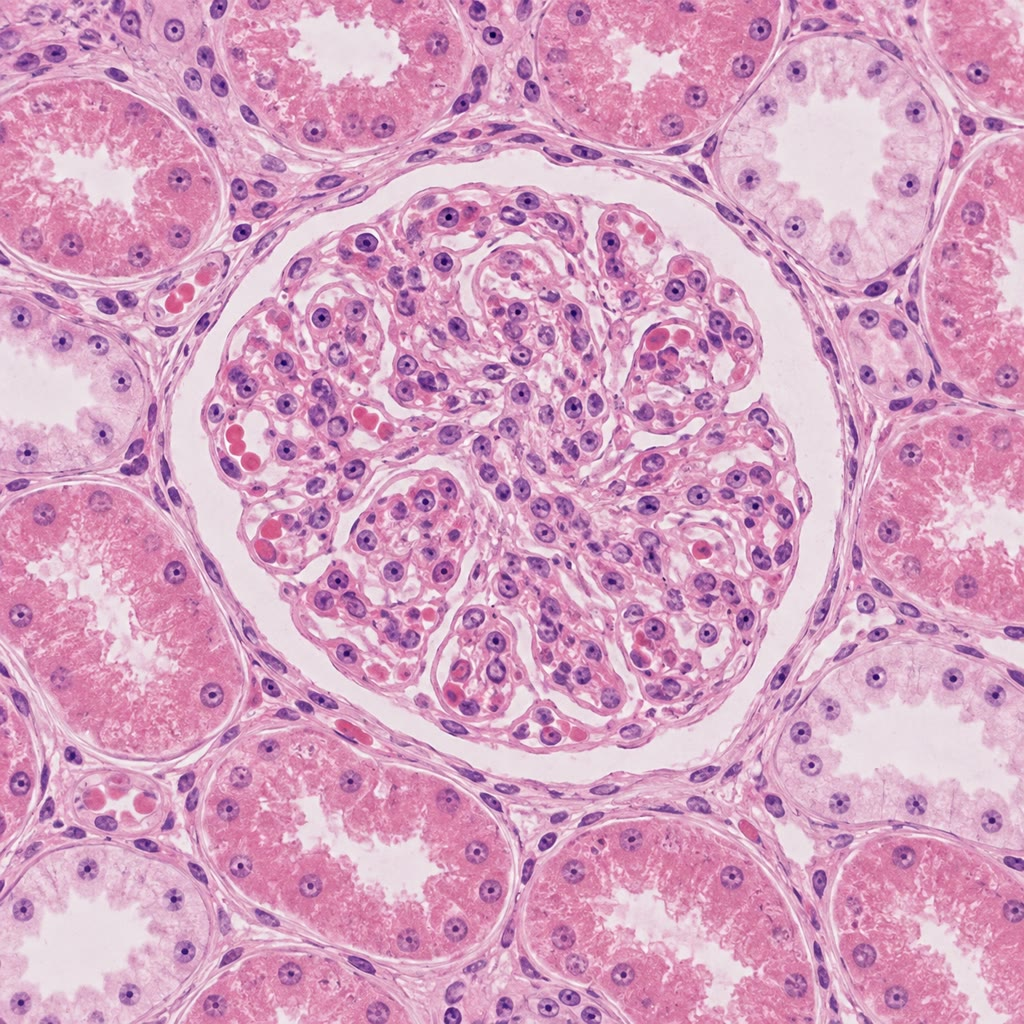
\includegraphics[width=0.46\linewidth]{images/book5/ai/b5-20-kidney-section.jpg}\hspace{0.04\linewidth}
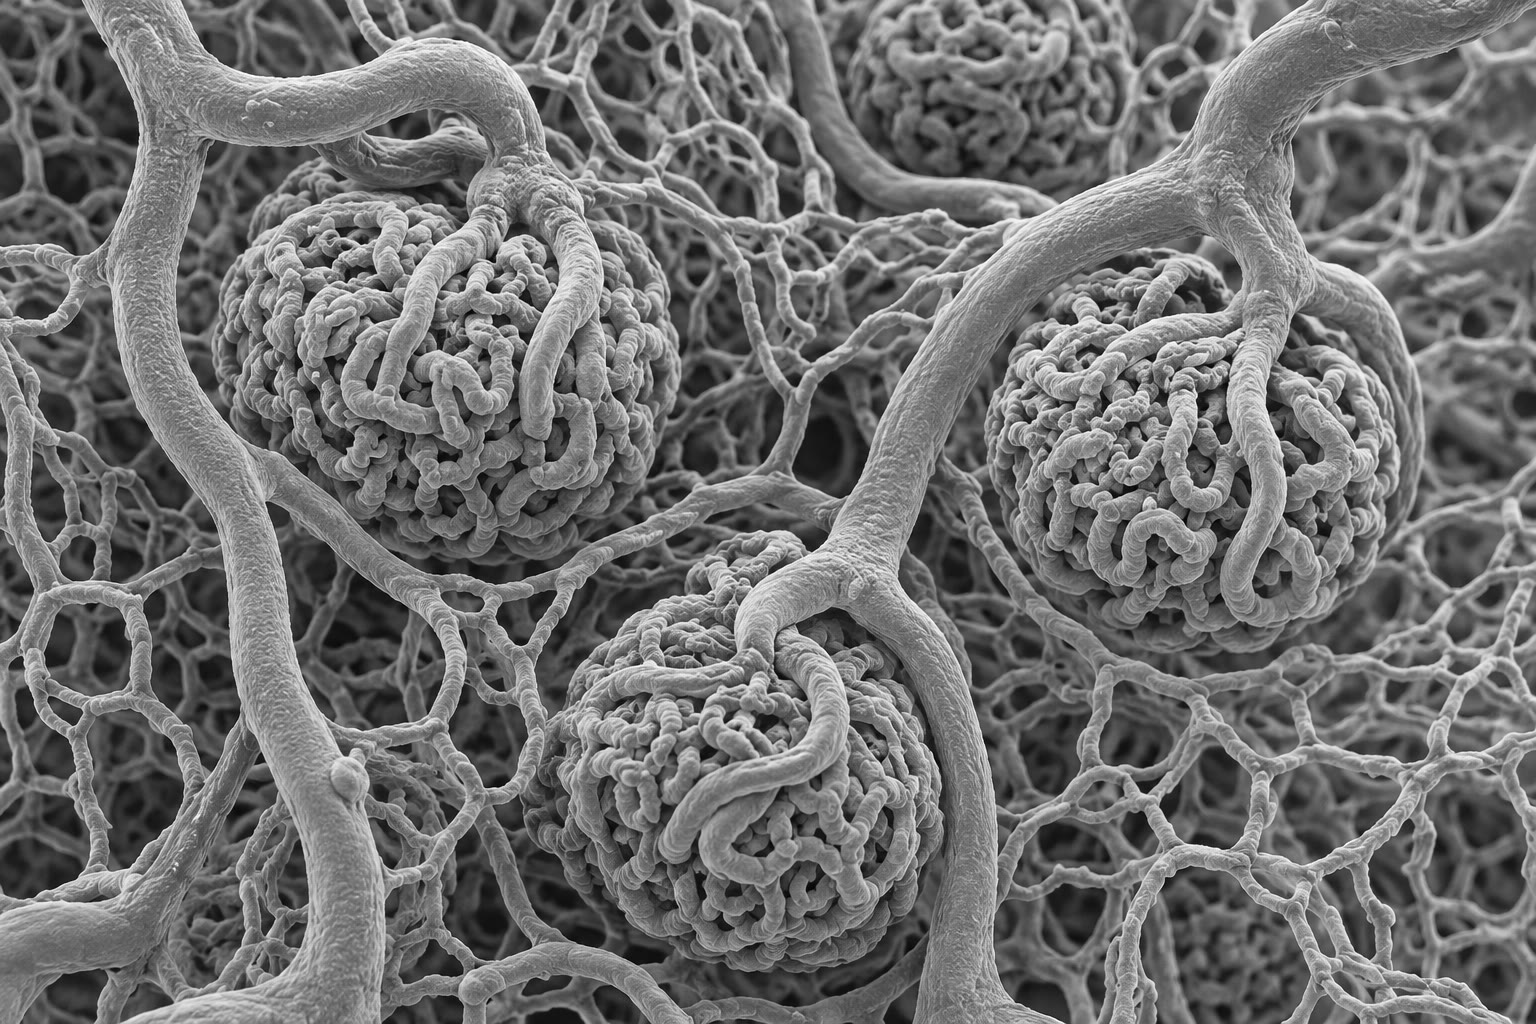
\includegraphics[width=0.46\linewidth]{images/book5/ai/b5-20-nephron-cast.jpg}

{\small बाएँ: काट में वृक्क वल्कुट --- समीपस्थ तथा दूरस्थ नलिकाओं की
आकृतियों के बीच अपने संपुट में बैठा कोई \omterm{def:b3:renal-osmoregulation:nephron}{केशिकागुच्छ}। दाएँ: वल्कुट का
कोई वाहिकीय ढाँचा, जिसमें ऊन का हर गोला परिनलिकीय केशिकाओं के बीच अपनी
अभिवाही तथा अपवाही वाहिकाओं के साथ कोई \omterm{def:b3:renal-osmoregulation:nephron}{केशिकागुच्छ} है।}
\end{omfigure}

\section{दूसरे प्राणी, दूसरे हल}

\begin{definition}[प्राणियों भर में परासरण-नियमन]\label{def:b3:renal-osmoregulation:comparative}
\index{मैल्पीघी नलिका}\index{लवण ग्रंथि}\index{क्लोराइड कोशिका}\index{उपापचयी जल}\index{सापेक्ष मज्जा-मोटाई}
मीठे पानी की मछलियाँ ऐसे माध्यम में रहती हैं जिसकी \omterm{def:b3:renal-osmoregulation:problem}{परासरणीयता} उनके
रक्त की दसवाँ भाग है: जल क्लोमों से होकर भीतर भर जाता है, नमक रिसकर
निकलता है, और वे भरपूर तनु मूत्र निकालती हैं तथा क्लोमों की
\emph{क्लोराइड कोशिकाओं} से नमक सक्रिय रूप से भीतर लेती हैं, कभी पीती
नहीं। समुद्री अस्थिमीन, जिनका रक्त समुद्र की \omterm{def:b3:renal-osmoregulation:problem}{परासरणीयता} का तिहाई है,
क्लोमों से जल खोती हैं, समुद्री जल पीती हैं, और उन्हीं क्लोराइड
कोशिकाओं को उलटा चलाकर नमक बाहर पंप करती हैं, और मूत्र थोड़ा रखती हैं;
शार्क इसके बजाय यूरिया (और अपने प्रोटीनों को उससे बचाए रखने के लिए
ट्राइमेथिलऐमीन ऑक्साइड) रोककर अपना रक्त समुद्र के समपरासरणी रखती हैं,
और बचा नमक किसी गुदा-ग्रंथि से उत्सर्जित करती हैं। समुद्री पक्षी और
समुद्री सरीसृप आँखों के ऊपर \emph{लवण ग्रंथियाँ} ढोते हैं, जो समुद्र से
दुगुने नमकीन किसी खारे घोल का स्राव करती हैं, जिससे कोई अल्बाट्रॉस
समुद्र से पी सकता है। कीट रक्तचाप के बजाय सक्रिय पोटैशियम-स्राव से चलती
\emph{मैल्पीघी नलिकाओं} से छानते हैं, और मलाशय में जल इतनी पूरी तरह
पुनःसोख लेते हैं कि किसी रेगिस्तानी भृंग की बीट सूखी होती है। स्तनियों
में गाढ़ा करने की शक्ति पाशों की लंबाई के साथ, गुर्दे के आकार के सापेक्ष
(यानी \emph{सापेक्ष मज्जा-मोटाई} के साथ), बढ़ती है: कोई ऊदबिलाव
\qty{500}{mOsm/L} तक जाता है, कोई मनुष्य \num{1200}, कोई ऊँट \num{3000},
और कंगारू चूहा \num{5500} --- जिससे वह उस \emph{उपापचयी जल} पर जी लेता
है जो उसका भोजन ऑक्सीकृत होने पर छोड़ता है, यानी प्रति ग्राम स्टार्च
लगभग \qty{0.6}{g} जल, और साथ में ऐसी नाक जो प्रतिधारा शीतलन से हर छोड़ी
गई साँस का जल वापस पा लेती है।
\end{definition}

\begin{omfigure}
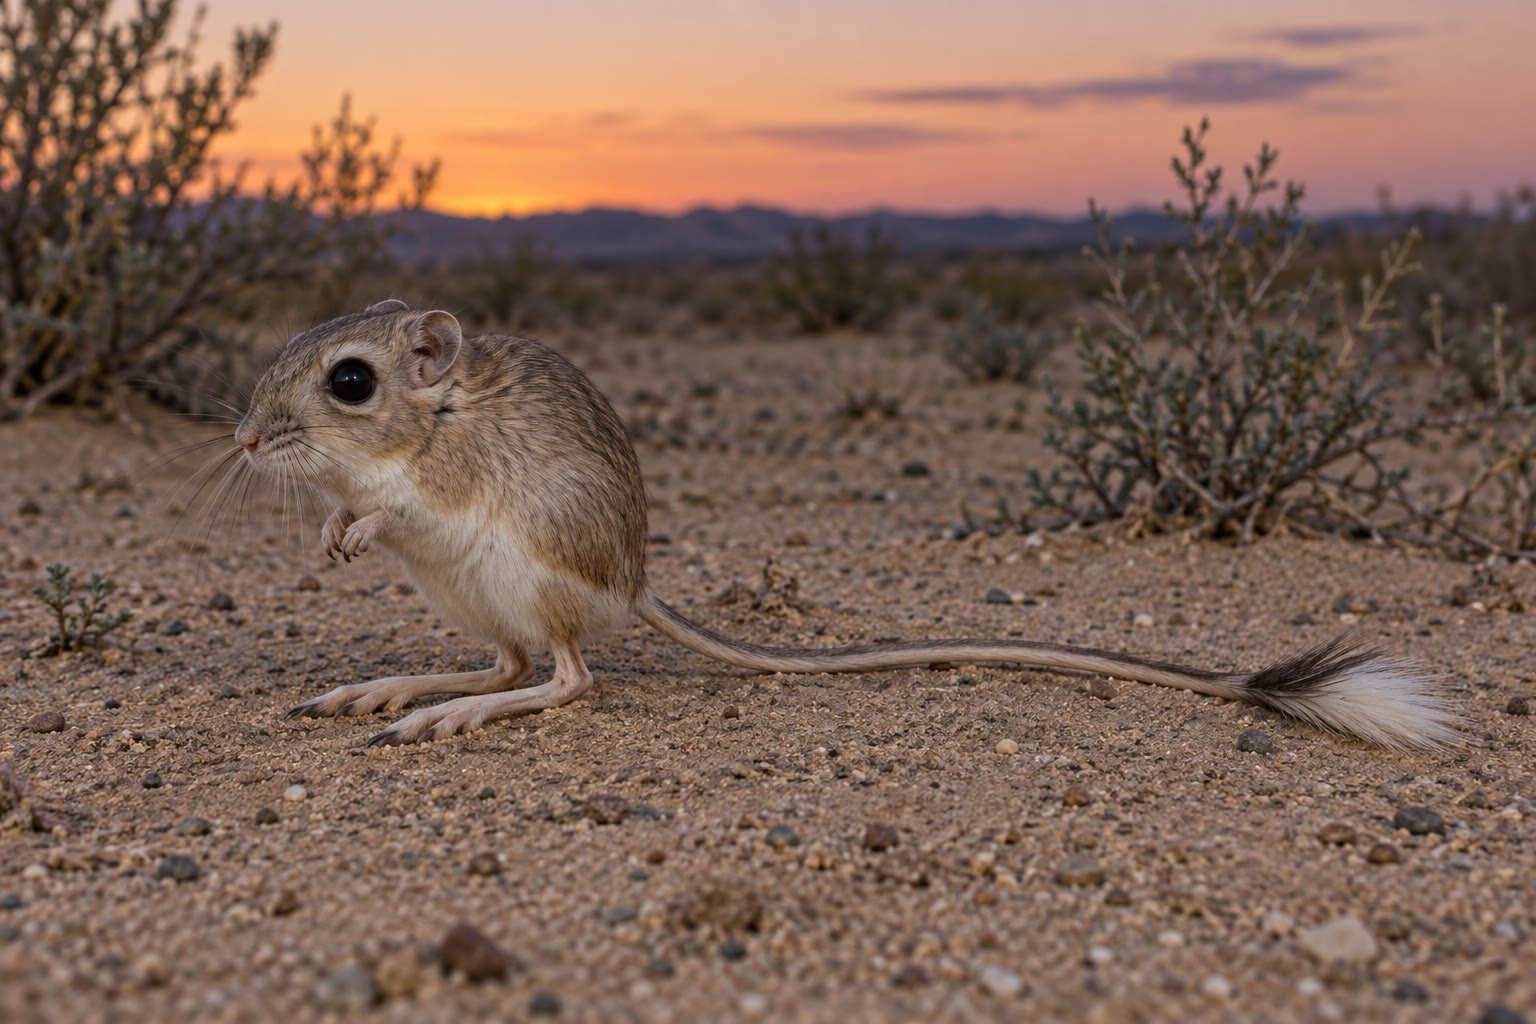
\includegraphics[width=0.56\linewidth]{images/book5/ai/b5-20-kangaroo-rat.jpg}

{\small कोई कंगारू चूहा, जो कभी पीता नहीं: हेनले के लंबे पाश, समुद्री
जल से पाँच गुना गाढ़ा मूत्र, कोई ठंडी नाक जो हर साँस का जल संघनित कर
लेती है, और ऐसा आहार जिसका ऑक्सीकरण उसका सारा ज़रूरी जल बना देता है।}
\end{omfigure}

\begin{remark}[अभिकल्प-समस्या के रूप में गुर्दा]\label{rem:b3:renal-osmoregulation:design}
स्तनी गुर्दा दिन भर में प्लाज़्मा के आयतन से चालीस गुना छानता है, केवल
इसलिए कि उसका लगभग सारा वापस ले ले: कोई फ़िज़ूलख़र्च अभिकल्प, जिसकी बात
यह है कि सब कुछ छानकर चुन-चुनकर पुनःसोखना हर उस कचरे को, जो कभी भी
प्रकट हो सकता है, चुन-चुनकर स्रवित करने से सरल है। उसकी कीमत विश्रामी
उपापचय का वह \qty{7}{\%} है जो सोडियम वापस पंप करने में जाता है, और
उसकी दुर्बलता वह नाज़ुक छन्ना है, जो ऊँचे दाब और ऊँचे ग्लूकोस के तहत
धीरे-धीरे विफल होता है। उसकी चतुराई वह प्रतिधारा पाश है, जो गहरी
मछलियों के तैर-मूत्राशयों में, बगुले-सरीखे पक्षियों की टाँगों में और
रेगिस्तानी कृंतकों की नाकों में भी मिलता है, और जिससे कोई छोटा, वहन
करने लायक स्थानीय अंतर किसी बड़े में चुन दिया जाता है --- हर बार वही
विचार, कि प्रवाह से कोई प्रवणता बनाई जा सकती है।
\end{remark}

\section{अभ्यास}

\begin{exercise}[$\star$]\label{exo:b3:renal-osmoregulation:1}
\omterm{def:b3:renal-osmoregulation:nephron}{वृक्काणु} के खंड क्रम से बताइए और हर एक जो करता है उसमें से एक बात।
\end{exercise}

\begin{exercise}[$\star$]\label{exo:b3:renal-osmoregulation:2}
निकासी परिभाषित कीजिए। किसी पदार्थ की प्लाज़्मा सांद्रता
\qty{2}{mg/mL} है, मूत्र-सांद्रता \qty{100}{mg/mL} और मूत्र-प्रवाह
\qty{1.5}{mL/min}। उसकी निकासी निकालिए और बताइए कि वह पुनःसोखा जाता है,
स्रवित होता है, या कुछ भी नहीं, यदि GFR \qty{120}{mL/min} हो।
\end{exercise}

\begin{exercise}[$\star$]\label{exo:b3:renal-osmoregulation:3}
कोई मीठे पानी की मछली कभी क्यों नहीं पीती और कोई समुद्री मछली लगातार
क्यों पीती है? हर एक में क्लोम क्या करते हैं?
\end{exercise}

\begin{exercise}[$\star$]\label{exo:b3:renal-osmoregulation:4}
हेनले के पाश का \omterm{prop:b3:renal-osmoregulation:countercurrent}{एकल प्रभाव} क्या है, उसे कौन-सी भुजा बनाती है, और दोनों
भुजाओं की जल-पारगम्यता भिन्न क्यों होनी चाहिए?
\end{exercise}

\begin{exercise}[$\star\star$]\label{exo:b3:renal-osmoregulation:5}
केशिकागुच्छी केशिका का दाब \qty{60}{mmHg}, बोमन-अवकाश का
\qty{18}{mmHg}, प्लाज़्मा का कलिलाकर्षी दाब अभिवाही सिरे पर
\qty{28}{mmHg}, जो अपवाही सिरे पर चढ़कर \qty{35}{mmHg} हो जाता है। हर
सिरे पर शुद्ध निस्यंदन दाब निकालिए और समझाइए कि निस्यंदन उस केशिका के
अंत से पहले क्यों रुक सकता है। GFR पर प्लाज़्मा प्रवाह के असर के लिए
इससे क्या निकलता है?
\end{exercise}

\begin{exercise}[$\star\star$]\label{exo:b3:renal-osmoregulation:6}
किसी रोगी की क्रिएटिनिन निकासी \qty{40}{mL/min} है। प्लाज़्मा सोडियम
\qty{140}{mmol/L} है, मूत्र सोडियम \qty{70}{mmol/L}, मूत्र-प्रवाह
\qty{1}{mL/min}। सोडियम का छना भार, उत्सर्जन, पुनःसोखा गया अंश, और
सोडियम की निकासी निकालिए।
\end{exercise}

\begin{exercise}[$\star\star$]\label{exo:b3:renal-osmoregulation:7}
कोई व्यक्ति ऐसा आहार लेता है जो दिन भर में \qty{900}{mOsm} विलेय बनाता
है और वह \qty{1200}{mOsm/L} तक गाढ़ा कर सकता है। न्यूनतम मूत्र-आयतन?
यदि वृक्क रोग अधिकतम को \qty{400}{mOsm/L} तक गिरा दे, तो संतुलन में
रहने के लिए उसे कितना पीना पड़ेगा, \qty{0.9}{L} की अगोचर हानि मानते हुए?
\end{exercise}

\begin{exercise}[$\star\star$]\label{exo:b3:renal-osmoregulation:8}
इनमें मूत्र के आयतन तथा \omterm{def:b3:renal-osmoregulation:problem}{परासरणीयता}, प्लाज़्मा सोडियम और प्यास की दशा
का पूर्वानुमान कीजिए: (क) डायबिटीज़ इन्सिपिडस, (ख) किसी \omterm{def:b3:cancer-biology:hallmarks}{अर्बुद} द्वारा
वैसोप्रेसिन का अनुचित स्राव, (ग) \omterm{def:b3:renal-osmoregulation:controls}{ऐल्डोस्टेरॉन} की अधिकता, (घ) हफ़्ते भर
बिना नमक का आहार।
\end{exercise}

\begin{exercise}[$\star\star$]\label{exo:b3:renal-osmoregulation:9}
\qty{300}{mOsm/L} के प्लाज़्मा के साथ, \qty{6}{mL/min} पर
\qty{100}{mOsm/L} के मूत्र के लिए और \qty{0.6}{mL/min} पर
\qty{1000}{mOsm/L} के मूत्र के लिए \omterm{prop:b3:renal-osmoregulation:water}{मुक्त-जल निकासी} निकालिए। हर एक की
व्याख्या कीजिए।
\end{exercise}

\begin{exercise}[$\star\star\star$]\label{exo:b3:renal-osmoregulation:10}
उस पाश को $n$ चरणों का प्रतिरूप दीजिए जिनमें हर चरण पर आरोही तरल
अंतराल से \qty{200}{mOsm/L} नीचे हो और अवरोही तरल उसके बराबर, और जिसमें
तरल \qty{300}{mOsm/L} पर घुसता हो। तर्क दीजिए कि मोड़ पर
स्थायी-अवस्था \omterm{def:b3:renal-osmoregulation:problem}{परासरणीयता} $300 +
200n$ के पास पहुँच सकती है, जिससे वह प्रवणता पाश की लंबाई और पंप के
\omterm{prop:b3:renal-osmoregulation:countercurrent}{एकल प्रभाव} से सीमित होती है, और बताइए कि $n$ भौतिक रूप से किससे तय होता
है।
\end{exercise}

\begin{exercise}[$\star\star\star$]\label{exo:b3:renal-osmoregulation:11}
कोई कंगारू चूहा दिन भर में \qty{5}{g} सूखा बीज खाता है, जिसका
\qty{80}{\%} स्टार्च है, जो CO$_{2}$ तथा जल में ऑक्सीकृत होता है (प्रति
ग्राम स्टार्च \qty{0.6}{g} जल)। उसे दिन भर में \qty{3}{mOsm} विलेय
\qty{5500}{mOsm/L} पर उत्सर्जित करना पड़ता है, और वह दिन भर में
\qty{1.5}{g} जल किसी ऐसी नाक से वाष्पन द्वारा खोता है जो अपनी साँस का
\qty{70}{\%} जल वापस पा लेती है। उसका जल-बजट तोलिए और बताइए कि क्या वह
बिना पिए जी लेता है।
\end{exercise}

\begin{exercise}[$\star\star\star$]\label{exo:b3:renal-osmoregulation:12}
अपोहन में रक्त किसी झिल्ली के एक ओर और अपोहक-द्रव दूसरी ओर, प्रतिधारा
में, बहते हैं। समझाइए कि प्रतिधारा प्रवाह समांतर प्रवाह से अधिक निकासी
क्यों करता है, ऐसी किसी मशीन की निकासी आँकिए जो \qty{300}{mL/min} रक्त
से \qty{70}{\%} दक्षता के साथ यूरिया हटाती है, और हफ़्ते भर में दो
गुर्दों से तुलना कीजिए, यदि वह मशीन हफ़्ते में तीन बार चार-चार घंटे
चले।
\end{exercise}

\section{समस्या: दिन भर में अठारह बाल्टियाँ}

\begin{problem}[{सप्तांत समस्या --- केशिकागुच्छ से मूत्राशय तक पीछा
किया गया दिन भर का निस्यंद: स्टार्लिंग दाब, चार पदार्थों की निकासियाँ,
ग्लूकोस की देहली, अधिकतम तनुकरण से समुद्री जल तक का जल-बजट, और किसी
रेगिस्तानी कृंतक का संतुलन, जिसका अंत GFR पर होता है, अनिवार्य
मूत्र-आयतन पर, और उस शुद्ध जल पर जो लीटर भर समुद्री जल देता है}]
\label{pb:b3:renal-osmoregulation:1}
आँकड़े: $K_{f} = \qty{12.5}{mL/min/mmHg}$; $P_{\text{GC}} = \qty{55}{mmHg}$,
$P_{\text{BS}} = \qty{15}{mmHg}$, $\pi_{\text{GC}} = \qty{30}{mmHg}$।
प्लाज़्मा: इनुलिन \qty{0.5}{mg/mL}, क्रिएटिनिन \qty{0.01}{mg/mL},
यूरिया \qty{5}{mmol/L}, ग्लूकोस \qty{5}{mmol/L},
पैरा-अमीनोहिप्यूरेट \qty{0.02}{mg/mL}, Na$^{+}$ \qty{140}{mmol/L},
\omterm{def:b3:renal-osmoregulation:problem}{परासरणीयता} \qty{290}{mOsm/L}। मूत्र-प्रवाह \qty{1}{mL/min}: इनुलिन
\qty{62.5}{mg/mL}, क्रिएटिनिन \qty{1.3}{mg/mL}, यूरिया
\qty{250}{mmol/L}, ग्लूकोस $0$, पैरा-अमीनोहिप्यूरेट \qty{13}{mg/mL},
Na$^{+}$ \qty{100}{mmol/L}, \omterm{def:b3:renal-osmoregulation:problem}{परासरणीयता} \qty{600}{mOsm/L}। हीमैटोक्रिट
$0.45$। ग्लूकोस का $T_{m} =
\qty{375}{mg/min}$ (\qty{2.1}{mmol/min})। दैनिक विलेय \qty{600}{mOsm};
$U_{\max} = \qty{1200}{mOsm/L}$, $U_{\min} = \qty{50}{mOsm/L}$;
अगोचर हानि \qty{0.9}{L/d}; समुद्री जल \qty{1000}{mOsm/L}।

\medskip
\noindent\textbf{भाग I --- छन्ना।}
\begin{enumerate}
  \item शुद्ध निस्यंदन दाब और GFR निकालिए।
  \item GFR को लीटर प्रति दिन में बदलिए। प्लाज़्मा का आयतन
        (\qty{3}{L}) कितनी बार छना जाता है?
  \item इनुलिन की निकासी निकालिए और GFR से तुलना कीजिए। क्रिएटिनिन की
        निकासी निकालिए; वह थोड़ी बड़ी क्यों है?
  \item पैरा-अमीनोहिप्यूरेट की निकासी (यानी वृक्कीय प्लाज़्मा प्रवाह),
        वृक्कीय रक्त-प्रवाह, और निस्यंदन-अंश निकालिए।
  \item अपवाही अणुधमनी सिकुड़कर $P_{\text{GC}}$ को \qty{60}{mmHg} तक
        उठा देती है। नई GFR? वे औषधें, जो ऐंजियोटेंसिन~II रोकती हैं,
        किसी स्वस्थ गुर्दे में GFR थोड़ी क्यों गिरा देती हैं और किसी
        मधुमेही गुर्दे की रक्षा क्यों करती हैं?
  \item मूत्र में \qty{3}{g/d} पर प्रोटीन प्रकट होता है। उस छन्ने की
        कौन-सी परत विफल हुई है, और यह चलता रहे तो प्लाज़्मा के
        कलिलाकर्षी दाब का तथा ऊतकों का क्या होता है?
\end{enumerate}

\medskip
\noindent\textbf{भाग II --- सँभाल।}
\begin{enumerate}[resume]
  \item यूरिया: छना भार, उत्सर्जन, पुनःसोखा गया अंश, और निकासी।
  \item सोडियम: दिन भर का छना भार मोलों तथा ग्रामों में, उत्सर्जन, और
        पुनःसोखा गया अंश। यदि कुछ भी पुनःसोखा न जाता तो दिन भर में
        कितने किलोग्राम नमक खो जाता?
  \item ग्लूकोस: छना भार mmol/min में और ग्राम प्रति दिन में; क्या कुछ
        उत्सर्जित होता है? किस प्लाज़्मा ग्लूकोस पर छना भार
        $T_{m}$ तक पहुँचता है (यानी देहली)?
  \item किसी मधुमेही का प्लाज़्मा ग्लूकोस \qty{20}{mmol/L} है। प्रति
        मिनट और प्रति दिन ग्रामों में उत्सर्जित ग्लूकोस, और अतिरिक्त
        मूत्र-आयतन, यदि ग्लूकोस का हर \qty{300}{mOsm} प्रचलित सांद्रता
        पर \qty{1}{L} ढोता हो। अनुपचारित मधुमेह की प्यास और भार-हानि
        समझाइए।
  \item सोडियम पुनःसोखने की लागत प्रति तीन Na$^{+}$ एक ATP है। गुर्दा
        दिन भर में सोडियम पर ATP के कितने मोल खर्च करता है, और कितने
        किलोजूल (\qty{50}{kJ/mol})? विश्रामी \qty{7}{MJ/d} से तुलना
        कीजिए।
  \item समझाइए कि गुर्दा हर कचरे को स्रवित करने के बजाय छानता तथा
        पुनःसोखता क्यों है, इस हिसाब से कि उस नलिका को क्या-क्या
        पहचानना पड़ता।
\end{enumerate}

\medskip
\noindent\textbf{भाग III --- जल।}
\begin{enumerate}[resume]
  \item आँकड़ों से परासरणी निकासी $U_{\text{osm}}V/P_{\text{osm}}$, और
        \omterm{prop:b3:renal-osmoregulation:water}{मुक्त-जल निकासी}। क्या वह व्यक्ति जल बचा रहा है या बहा रहा है?
  \item दिन भर के विलेय के लिए न्यूनतम मूत्र-आयतन; अधिकतम
        ($U_{\min}$ पर); और अगोचर हानि के साथ, न्यूनतम पर दिन भर की
        कुल जल-ज़रूरत।
  \item लीटर भर समुद्री जल पिया जाता है। उसका नमक $U_{\max}$ पर
        उत्सर्जित करने के लिए कितना मूत्र चाहिए, और उस दिन के अपने
        विलेय को गिनने से पहले शुद्ध जल-लाभ क्या है? गिनने के बाद?
  \item वैसोप्रेसिन नहीं है (डायबिटीज़ इन्सिपिडस) और मूत्र
        $U_{\min}$ पर ही रहता है। उसी विलेय के लिए दिन भर का
        मूत्र-आयतन, और संतुलन बनाए रखने के लिए रोज़ कितना जल पीना
        पड़ेगा।
  \item \qty{20}{mOsm/L} की बियर: गुर्दा, $U_{\min}$ पर, जब वह जल
        उत्सर्जित न कर सके, उससे पहले दिन भर में कितनी पी जा सकती है?
        (जो जल $U_{\min}$ पर उस विलेय के ढोने से अधिक हो वह जमा हो
        जाता है।)
  \item बिना जल की एक रात के बाद प्लाज़्मा की \omterm{def:b3:renal-osmoregulation:problem}{परासरणीयता}
        \qty{298}{mOsm/L} है। वह कितने प्रतिशत चढ़ी, और अधश्चेतक क्या
        करता है? यदि कुल देह-जल \qty{42}{L} हो और विलेय अपरिवर्तित, तो
        जल की कमी आँकिए।
  \item समझाइए कि नमक पसीने में खोता हुआ कोई मैराथॉन धावक, जो
        \qty{6}{L} जल पी ले, ख़तरनाक रूप से कम प्लाज़्मा सोडियम तक कैसे
        पहुँच सकता है, और उसे रोकने के लिए गुर्दे को क्या करना पड़ता।
\end{enumerate}

\medskip
\noindent\textbf{भाग IV --- रेगिस्तान।}
\begin{enumerate}[resume]
  \item कोई कंगारू चूहा दिन भर में \qty{3}{mOsm} \qty{5500}{mOsm/L} पर
        उत्सर्जित करता है। मूत्र-आयतन? उसी विलेय के लिए किसी मानव
        गुर्दे को अपनी अधिकतम पर जितना आयतन चाहिए होता, उससे तुलना
        कीजिए।
  \item उसका भोजन दिन भर में \qty{2.4}{g} \omterm{def:b3:renal-osmoregulation:comparative}{उपापचयी जल} देता है और वह
        साँस से \qty{1.6}{g} तथा मल में \qty{0.3}{g} खोता है। प्रश्न 20
        के मूत्र के साथ उसका बजट तोलिए।
  \item कोई ऊँट \qty{3000}{mOsm/L} तक गाढ़ा करता है और अपने देह-जल का
        \qty{25}{\%} खोना सह लेता है। \qty{65}{\%} जल वाले किसी
        \qty{500}{kg} ऊँट के लिए, वह कितना खो सकता है, और
        \qty{5}{L/d} की हानि पर वह कितने दिन चलता है?
  \item कोई समुद्री पक्षी दिन भर में \qty{200}{g} मछली खाता है और
        \qty{100}{mL} समुद्री जल पीता है, जिससे उसमें \qty{150}{mmol}
        NaCl जाता है। उसकी \omterm{def:b3:renal-osmoregulation:comparative}{लवण ग्रंथि} \qty{800}{mmol/L} पर स्राव करती
        है। वह कितना खारा घोल बनाता है, और इसके लिए वह ग्रंथि उस
        गुर्दे से बेहतर क्यों है (जो पक्षियों में केवल \qty{600}{mOsm/L}
        तक गाढ़ा करता है)?
  \item \qty{100}{g} की कोई मीठे पानी की मछली दिन भर में अपने क्लोमों
        से अपने देह-द्रव्यमान का \qty{30}{\%} जल पा लेती है। उसे कितना
        मूत्र बनाना पड़ता है, अपने रक्त के सापेक्ष किस \omterm{def:b3:renal-osmoregulation:problem}{परासरणीयता} पर,
        और सक्रिय ग्रहण के बिना उसके नमक का क्या होता?
  \item सारांश दीजिए: GFR (प्रश्न~1), अनिवार्य मूत्र-आयतन (प्रश्न~14),
        और लीटर भर समुद्री जल से मिलता शुद्ध जल, उस दिन का विलेय गिनने
        के बाद (प्रश्न~15)।
\end{enumerate}
\end{problem}
